\documentclass{article}
\usepackage{pgfplots}
 \pgfplotsset{compat=newest}

 \begin{document}

Introduction

The number of Large Language Models (LLM) grew considerably and seems to provide new challenges for processor and compiler developers on a daily basis. The main challenge is to improve the performance of an LLM within the constraints of already existing hardware. Although hardware accelerators entering the market in relative rapid succession, companies may not be willing to upgrade their compute ressources with each new generation of processors. Usually a software upgrade and tool upgrade is much more common compared to a hardware and processor upgrade.  
There are essentially two areas, which are targeted to improve performance. First there is the improvement of the hardware by utilizing new hardware architectures and improving existing hardware architecture by adding specific features which benefit neural networks. The other area is the improvement by software tools. Specifically AI compilers are under development, which both exising hardware better. These optimizations are often in the area of parallel execution of workloads, faster data transfer between nodes and faster loading of components into the hardware to name a few. 
One upcoming are in the optimization arena is the fusion of multiple neural network nodes into one single node. This paper discusses the fusion of a avgpool operation with the gelu operation and provides some measurements presenting the potential improvements of operator fusion.

Motivation 

A neural network workload constitutes of many nodes which mostly are executed individually or in eager mode. This means even with accelerating hardware, each node is executed on an individual basis and therefore the data is loaded in and out of the accelerator after each operation. A huge amount of data may be loaded to the accelerator, which then in a very aggressive highly parallel effort, performs such an operation to then load the result of said operation back to the host processor. A second node is processed in the exact same way, which means that the same or maybe a reduced or enlarged amount of data is loaded into the accelerator and the appropriate process is performed again. The neverthless means that data which might as well be processed within the same hardware is uploaded and downloaded between processing steps albeit being already at the correct location or stored in the correct memory.  
Fusion of nodes removed that additional upload and download step of interim results and performs the appropriate of two or more steps directly, i.e. multiple operations are fused together. This more often than not leads to a considerable improvement in throughput and performance of the exact same model. We can see this specifically in the combination of matrix multiplication with immediately following activation functions. The optimization of matrix multiplication and the fusion thereof with activation functions seems to be already widely discussed. In this paper we discuss another combination of operations, which are very common in the context of Large Language Models. The first is the avgPool2D function and the second is the gelu function. 

The approach
A three step process was executed to compare the runtime of a avgpool operation and a gelu operation. First the model was performed on a CPU using C++, then individual kernels were developed for the two operations, which ran back to back. And then a fused kernel was run to compare with the other runtimes. The following formulae show the what is implemented. 
Specifically the 2D embodiment of the avgpool operation was implemented as the following formula shows:
 


\(avgPool2D(N_i, C_j, h, w)  = \frac{1}{kH * kW} \sum_{m=0}^{kH-1} \sum_{n=0}^{kW-1}
                               input(N_i, C_j, stride[0] \times h + m, stride[1] \times w + n)\)


In addition to that the following gelu operation was implemented in a kernel. The kernel does not perform any of the published optimizations and simplifications for gelu. 


\( GELU(x) = 0.5 * x * (1 + \tanh(\sqrt{2 / \pi} * (x + 0.044715 * x^3)))\)



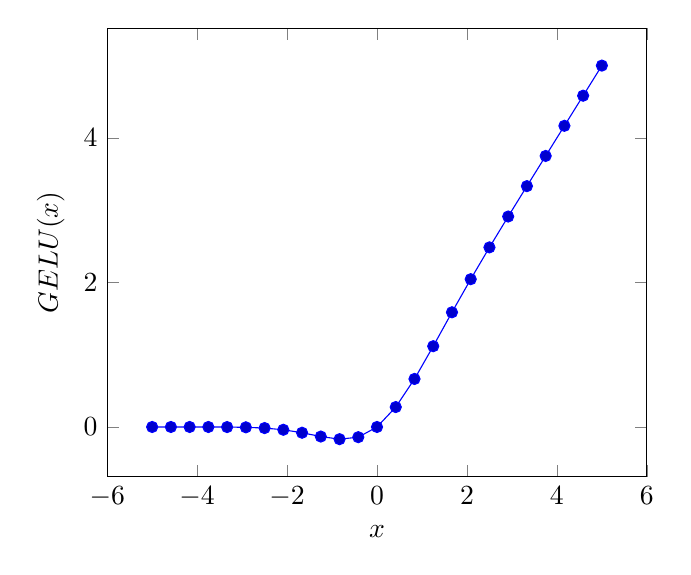
\begin{tikzpicture}

  \begin{axis}[ 
    xlabel=$x$,
    ylabel={$GELU(x)$}
  ] 
    \addplot {0.5 * x * (1 + tanh(sqrt(2/pi) * (x +0.044715 * x*x*x))) }; 
  \end{axis}

\end{tikzpicture}

The first result is based on a CPU implementation of avgPool2D with Gelu in C++ on a PC. There are again two parts to it, one is to run the avgPool2D stand alone and then add the Gelu portion. 



\begin{tikzpicture}
\begin{axis}[
    title=avgpool on CPU,
    xlabel={$dx$},
    ylabel={$sec$},
    legend entries={$dy=512$,$dy=1024$,$dy=1536$,$dy=2048$,$dy=2560$, $dy=3072$},
    legend pos=north west,
]
    \addplot [red] table {cpu_avgPool_dimi_512.dat};
    \addplot [blue] table {cpu_avgPool_dimi_1024.dat};
    \addplot [green] table {cpu_avgPool_dimi_1536.dat};
    \addplot [orange] table {cpu_avgPool_dimi_2048.dat};
    \addplot [magenta] table {cpu_avgPool_dimi_2560.dat};
    \addplot [yellow] table {cpu_avgPool_dimi_3072.dat};

\end{axis}
\end{tikzpicture}


\begin{tikzpicture}
\begin{axis}[
    title=avgpool with gelu on CPU,
    xlabel={$dx$},
    ylabel={$sec$},
    legend entries={$dy=512$,$dy=1024$,$dy=1536$,$dy=2048$,$dy=2560$, $dy=3072$},
    legend pos=north west,
]
    \addplot [red] table {cpu_avgPoolGelu_dimi_512.dat};
    \addplot [blue] table {cpu_avgPoolGelu_dimi_1024.dat};
    \addplot [green] table {cpu_avgPoolGelu_dimi_1536.dat};
    \addplot [orange] table {cpu_avgPoolGelu_dimi_2048.dat};
    \addplot [magenta] table {cpu_avgPoolGelu_dimi_2560.dat};
    \addplot [yellow] table {cpu_avgPoolGelu_dimi_3072.dat};

\end{axis}
\end{tikzpicture}


\begin{tikzpicture}
\begin{axis}[
    title=avgpool with and without gelu on CPU,
    xlabel={$dx$},
    ylabel={$sec$},
    legend entries={$only avgpool$, $with gelu$},
    legend pos=north west,
]
    \addplot [red] table {cpu_avgPool_dimi_3072.dat};
    \addplot [blue] table {cpu_avgPoolGelu_dimi_3072.dat};

\end{axis}
\end{tikzpicture}

It is showing that exercising Gelu on a CPU does not significantly change the overall runtime. The main explanation is that there is no additional allocation of memory involved. 

The following show the same for a CUDA kernel implementation. 

\begin{tikzpicture}
\begin{axis}[
    title=avgpool on CUDA,
    xlabel={$dx$},
    ylabel={$sec$},
    legend entries={$dy=512$,$dy=1024$,$dy=1536$,$dy=2048$,$dy=2560$, $dy=3072$},
    legend pos=north east,
]
    \addplot [red] table {cuda_avgPool_dimi_512.dat};
    \addplot [blue] table {cuda_avgPool_dimi_1024.dat};
    \addplot [green] table {cuda_avgPool_dimi_1536.dat};
    \addplot [orange] table {cuda_avgPool_dimi_2048.dat};
    \addplot [magenta] table {cuda_avgPool_dimi_2560.dat};
    \addplot [yellow] table {cuda_avgPool_dimi_3072.dat};

\end{axis}
\end{tikzpicture}

The interesing part is now that the Gelu kernel seems to be mostly slower than the equivalent CPU version, mostly because it allocates its separate memory. 


\begin{tikzpicture}
\begin{axis}[
    title=gelu on CUDA,
    xlabel={$dx$},
    ylabel={$sec$},
    legend entries={$dy=512$,$dy=1024$,$dy=1536$,$dy=2048$,$dy=2560$, $dy=3072$},
    legend pos=north east,
]
    \addplot [red] table {cuda_Gelu_dimi_512.dat};
    \addplot [blue] table {cuda_Gelu_dimi_1024.dat};
    \addplot [green] table {cuda_Gelu_dimi_1536.dat};
    \addplot [orange] table {cuda_Gelu_dimi_2048.dat};
    \addplot [magenta] table {cuda_Gelu_dimi_2560.dat};
    \addplot [yellow] table {cuda_Gelu_dimi_3072.dat};

\end{axis}
\end{tikzpicture}



\begin{tikzpicture}
\begin{axis}[
    title=avgPool and gelu sequential CUDA,
    xlabel={$dx$},
    ylabel={$sec$},
    legend entries={$dy=512$,$dy=1024$,$dy=1536$,$dy=2048$,$dy=2560$, $dy=3072$},
    legend pos=north east,
]
    \addplot [red] table {cuda_avgPoolGelu_notMerged_512.dat};
    \addplot [blue] table {cuda_avgPoolGelu_notMerged_1024.dat};
    \addplot [green] table {cuda_avgPoolGelu_notMerged_1536.dat};
    \addplot [orange] table {cuda_avgPoolGelu_notMerged_2048.dat};
    \addplot [magenta] table {cuda_avgPoolGelu_notMerged_2560.dat};
    \addplot [yellow] table {cuda_avgPoolGelu_notMerged_3072.dat};

\end{axis}
\end{tikzpicture}



\begin{tikzpicture}
\begin{axis}[
    title=avgPool and gelu fused CUDA,
    xlabel={$dx$},
    ylabel={$sec$},
    legend entries={$dy=512$,$dy=1024$,$dy=1536$,$dy=2048$,$dy=2560$, $dy=3072$},
    legend pos=north east,
]
    \addplot [red] table {cuda_avgPoolGelu_merged_512.dat};
    \addplot [blue] table {cuda_avgPoolGelu_merged_1024.dat};
    \addplot [green] table {cuda_avgPoolGelu_merged_1536.dat};
    \addplot [orange] table {cuda_avgPoolGelu_merged_2048.dat};
    \addplot [magenta] table {cuda_avgPoolGelu_merged_2560.dat};
    \addplot [yellow] table {cuda_avgPoolGelu_merged_3072.dat};

\end{axis}
\end{tikzpicture}







\end{document}